Das System stellt seine Funktionalität über die WEKA-Libary zur Verfügung. Damit diese arbeiten kann, werden Algorithmen benötigt. 
Um eine dynamische Ergänzung der Algorithmen zu ermöglichen wird WEKA als Mikrokernel implementiert. 
So können die Algorithmen als interne Server, wenn benötigt, geladen werden und neue Algorithmen können hinzugefügt werden, ohne das der WEKA-Quellcode bearbeitet werden muss. 
Alle Anfragen an WEKA laufen dabei über eine Datenschnittstelle, welche verschiedene Funktionalitäten für den Client bereitstellt.
So kann die Datenschnittstelle zurückgeben, welche Algorithmen von einem bestimmten Datensatz unterstützt werden oder ob ein zu erstellendes Modell bereits in der Datenbank vorhanden ist. 
WEKA übernimmt die Berechnung eines Modells und die Auswertung eines Datensatzes (bzw. eines Algorithmus). 
Der Web-Server übernimmt die Rolle eines Adapters, welcher die REST-Anfragen des Clients auswertet und weitere Instruktionen einleitet.
\begin{figure}[h]
\centering
	\vspace{-5pt}
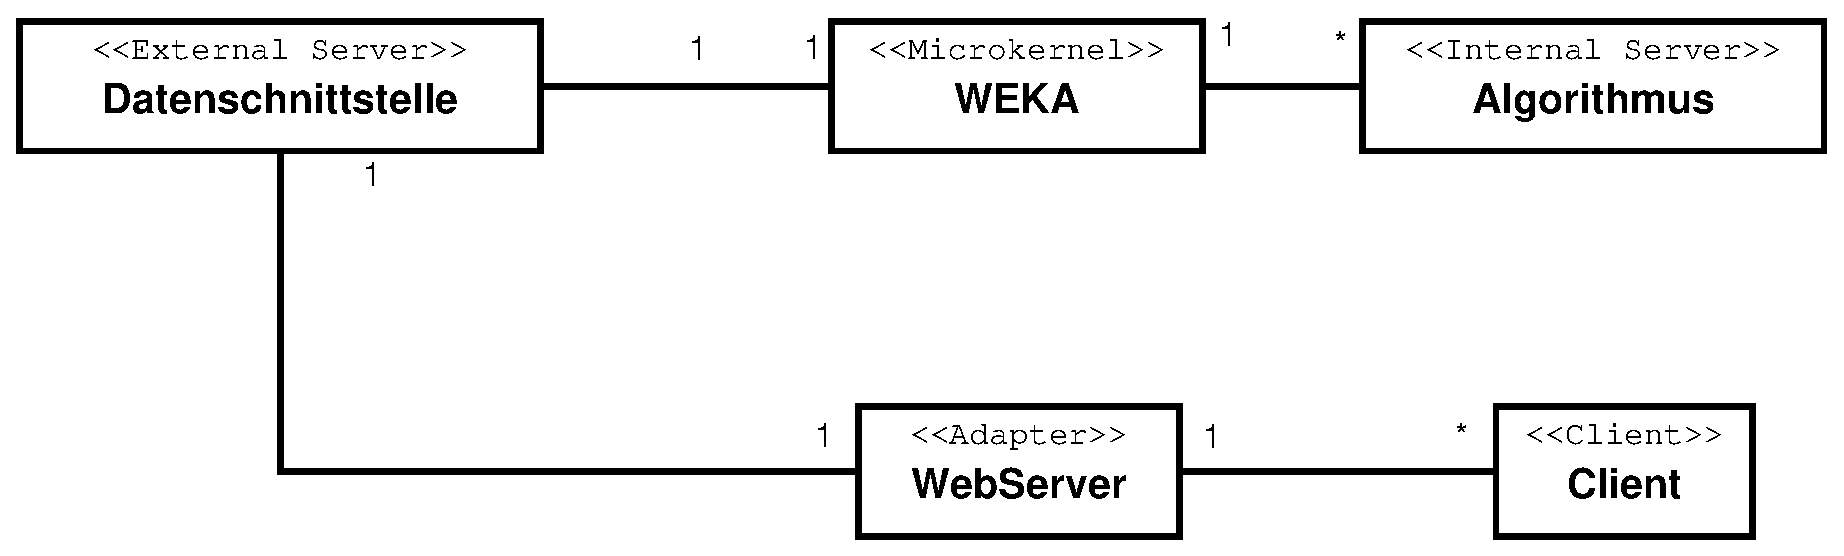
\includegraphics[width=0.7\linewidth]{Grafik/Diagramm/Microkernel}
\caption[Microkernel-Klassen]{Microkernel-Pattern mit WEKA}
\label{fig:Microkernel}
\end{figure}